\section{Pension System Reform in Argentina}\label{sec:argentina}\label{Argentina}

Argentina's expansion of pension coverage is the one change of pension design in this paper that actually took place, so it tests the model's prediction against an observed outcome before the model is used for counterfactuals. Argentina is a middle-income country with high labor informality, and its reform of 1994 tied full benefits to 30 years of contributions, which left about a third of those approaching retirement age in 2005 without full benefits.\footnote{The reform also let workers opt for a fully funded system, whose funds were nationalized in December 2008.} From 2005 a series of tax amnesties let workers with shorter contribution records draw a pension. They added 2.7 million beneficiaries (figure \ref{fig:Arg}) and raised the coverage of the elderly from 68\% to almost universal \parencite{CetrangoloG,Roffman}. Social security spending rose by 1.9\% of GDP between 2005 and 2010, of which 1.8\% of GDP was due to the amnesties \parencite{CetrangoloG}. Read as an increase in the universal pension $\epsilon$, the reform raises the equilibrium tax rate by enough to account for almost half of the rise due to the amnesties, and lowers savings and hours a little.

\begin{figure}[!htb]
\centering
\caption{Pension coverage in Argentina}
\label{fig:Arg}
\begin{threeparttable}
    \includegraphics[width=0.7\linewidth]{Figs/coverageArg.eps}
\begin{tablenotes}[flushleft]\footnotesize
    \item[] \textit{Note:} Number of social security beneficiaries, in millions. Source: Secretar\'ia de Seguridad Social and INDEC.
\end{tablenotes}
\end{threeparttable}
\end{figure}

\smalltitle{Calibration.}
We calibrate the model with informal savers to Argentina before the reforms, with informal households saving for retirement at the same return as formal ones, a model period of thirty years and 2010 as the calibration year. Table \ref{table:Arg:Calib} reports the result and appendix \ref{app:EPH} the household survey, the identifying formulas and the sources. The pre-reform $\epsilon = 0.29$ is the basic pension of retirees without a full contribution record, relative to the benefit of the least productive formal workers and discounted because it starts five to ten years after the formal retirement age, and $\gamma_0 = 0.32$ is the share of retirees on that pension before the reform \parencite{CetrangoloG}. The Bismarckian index $\theta = 0.84$ matches the observed ratio of replacement rates at mean and half-mean income. The reform raises $\epsilon$ to the universal level $\epsilon^U = 1-\theta+\theta\eta_1h_{t-1,1}/h_{t-1}$ of section \ref{sec:model}, at which informal retirees receive the benefit of the least productive formal ones. We impose a formal-sector capital share of $\alpha = 0.35$, between the values implied by the survey's informal earnings and by shadow-economy estimates of informal output, a Frisch elasticity of $\xi = 0.30$, and a ratio of workers to retirees $\nu_t$ from thirty-year gross population growth in census data and projections, as in \textcite{mkvss08}.

The remaining parameters are identified jointly with the equilibrium path. The formal productivities $\eta_i$ match the income distribution across the four formal quartiles of the survey, with a taste for leisure $X$ common to them whose level is pinned by the observed formal workweek of 42.5 hours.\footnote{Identifying one $X_i$ per quartile from the survey's relative hours instead makes hours data and leaves their average level unidentified (appendix \ref{app:EPH:vectorX}). Since $X$ enters no aggregate, only $\eta_i$ and $X_i$ differ, and every result of this section is the same under both.} Relative hours across quartiles are then a prediction, which reproduces the survey's ranking and overstates the hours of the top quartile, 1.18 against 1.10 times the formal average. Four parameters are solved against four targets in 2010: $\beta$ against a capital-output ratio of $3.23$, $\omega$ against an equivalent social security tax rate of 10.9\%, which is pension spending of 7.1\% of GDP before the 2001 crisis divided by the labor share of formal output, and $\eta_0$ and $X_0$ against the informal households' income and hours relative to the formal average.

%% GENERATED by python/paper/build.py from results/ -- do not edit by hand.
%% Rebuild:  .venv\Scripts\python.exe python\paper\build.py --only ArgentinaCalibration
%% Source:   results/paper/calibrationSummary.csv
\begin{table}[!htb]
\centering
\begin{threeparttable}
\caption{Calibration, Argentina}
\label{table:Arg:Calib}
\begin{tabular}{lll}
\toprule
\textbf{Parameter} & \textbf{Value} & \textbf{Target} \\
\midrule 
$\epsilon$ (\textit{pre}-reform) & $0.29$ & Minimum-to-full pension coverage \\[1ex] % row: epsilon
$\theta$ & $0.84$ & Replacement rate dispersion \\[1ex] % row: theta
$\alpha$ & $0.35$ & Factor income shares \\[1ex] % row: alpha
$\nu_t$ & $[1.65, 0.96]$ & 30-year gross population growth rates \\[1ex] % row: nu
$\xi$ & $0.30$ & Elasticity of labor supply \\[1ex] % row: xi
$\beta$ & $0.65$ & Capital--output ratio of $3.23$ \\[1ex] % row: beta
$X$ & $1.94$ & Average formal workweek of 42.5 hours \\[1ex] % row: X
$\eta_i$ & $[0.64, 0.90, 1.14, 1.87]$ & Income distribution \\[1ex] % row: eta
$\gamma_0$ & $0.32$ & Recipients of basic pension \\[1ex] % row: gamma0
$\omega$ & $1.49$ & Social security tax of $10.9\%$ \\[1ex] % row: omega
$\eta_0$ & $0.344$ & Informal relative income, eq.\ \eqref{eq:calibration_eta} \\[1ex] % row: eta0
$X_0$ & $0.804$ & Informal relative working hours \\[1ex] % row: X0
\bottomrule
\end{tabular}
\begin{tablenotes}[flushleft]
\footnotesize
\item[] \textit{Note:} Our default specification relies on $\rho=1$.
\end{tablenotes}
\end{threeparttable}
\end{table}


\smalltitle{The reform.}
Table \ref{table:Argentina:Universal} reports the effect in 2010 of an unanticipated and permanent rise of $\epsilon$ to $\epsilon^U$ under log-GHH preferences, first with the tax rate held at its pre-reform path and then chosen politically. The equivalent social security tax rate rises by 1.2 p.p., which at the labor share of formal output is pension spending of 0.8\% of GDP, almost half of the 1.8\% of GDP that the amnesties added. The reason for this is that the reform moves benefits toward informal retirees, who are poorer than formal ones and value benefits more at the margin, so retirees as a group support a larger system, as in proposition \ref{prop:LOG:PEE} for a large informal share. The savings rate falls by 0.3 p.p.\ of GDP and the average workweek by about 0.15 hours, the fall in savings in line with the estimate of \textcite{Ruffo} for the amnesty. Both responses come mainly from the tax: with the tax held fixed, the new claims dilute the benefits of formal households, who save more for retirement, so the savings rate rises by 0.2 p.p.\ of GDP and the workweek shortens by only 0.04 hours. The tax response builds over time, to 2.1 p.p.\ above the pre-reform path by 2040, because informal households, now covered, save less for retirement and as retirees demand more taxation.

%% GENERATED by python/paper/build.py from results/ -- do not edit by hand.
%% Rebuild:  .venv\Scripts\python.exe python\paper\build.py --only ArgentinaUniversal
%% Source:   results/shocks/{eeOnly,universal}_match_rho1.0000_commonX.csv
\begin{table}[!htb]
\centering
\begin{threeparttable}
\caption{Pension system reform, year 2010.}
\label{table:Argentina:Universal}
\begin{tabular}{lccc}
\toprule
\textbf{Scenario} & \textbf{Tax rate} & \textbf{Savings rate} & \textbf{Avg. workweek (hours)} \\
\midrule 
Baseline & 10.92\% & 14.40\% & 42.54 \\[1ex]
Economic Equilibrium & 10.92\% & 14.58\% & 42.50 \\[1ex]
Full effect & 12.17\% & 14.12\% & 42.39 \\[1ex]
\bottomrule
\end{tabular}
\begin{tablenotes}[flushleft]
\footnotesize
\item[] \textit{Note:} The reform permanently shifts $\epsilon = 1-\theta + \theta \eta_1 h_1/h$ at the calibration year, unanticipated. The ``Economic Equilibrium'' scenario solves for the new economic equilibrium path with taxes as in the Baseline scenario, but with the new permanent $\epsilon$; the ``Full effect'' scenario lets taxes be determined by the politico-economic equilibrium. $\rho=1$. The savings rate is savings relative to GDP.
\end{tablenotes}
\end{threeparttable}
\end{table}


Figure \ref{fig:Argentina_functionOfParams} shows the equilibrium in 2010 over a grid of designs $(\epsilon, \theta)$, each point an economy that has always had that design. The tax rate rises with $\epsilon$ and falls with $\theta$,\footnote{The signs are the same when informal households are hand-to-mouth, consistent with proposition \ref{prop:LOG:PEE} if $\gamma_0 > \bar{\gamma}_0$.} while the savings rate and the workweek fall with $\epsilon$ and rise with $\theta$, and the savings of informal relative to formal households fall with $\epsilon$. Between the two markers, the pre-reform calibration and the universal system at the calibrated $\theta$, the tax rate rises by about 2.0 p.p., more than the 1.2 p.p.\ on impact, because the savings of informal households have adjusted to the universal system; the difference is close to the long-run effect of the reform.

\begin{figure}[!htb]
\centering
\caption{Key variables as functions of $\epsilon, \theta$, year 2010}
\label{fig:Argentina_functionOfParams}
\begin{threeparttable}
    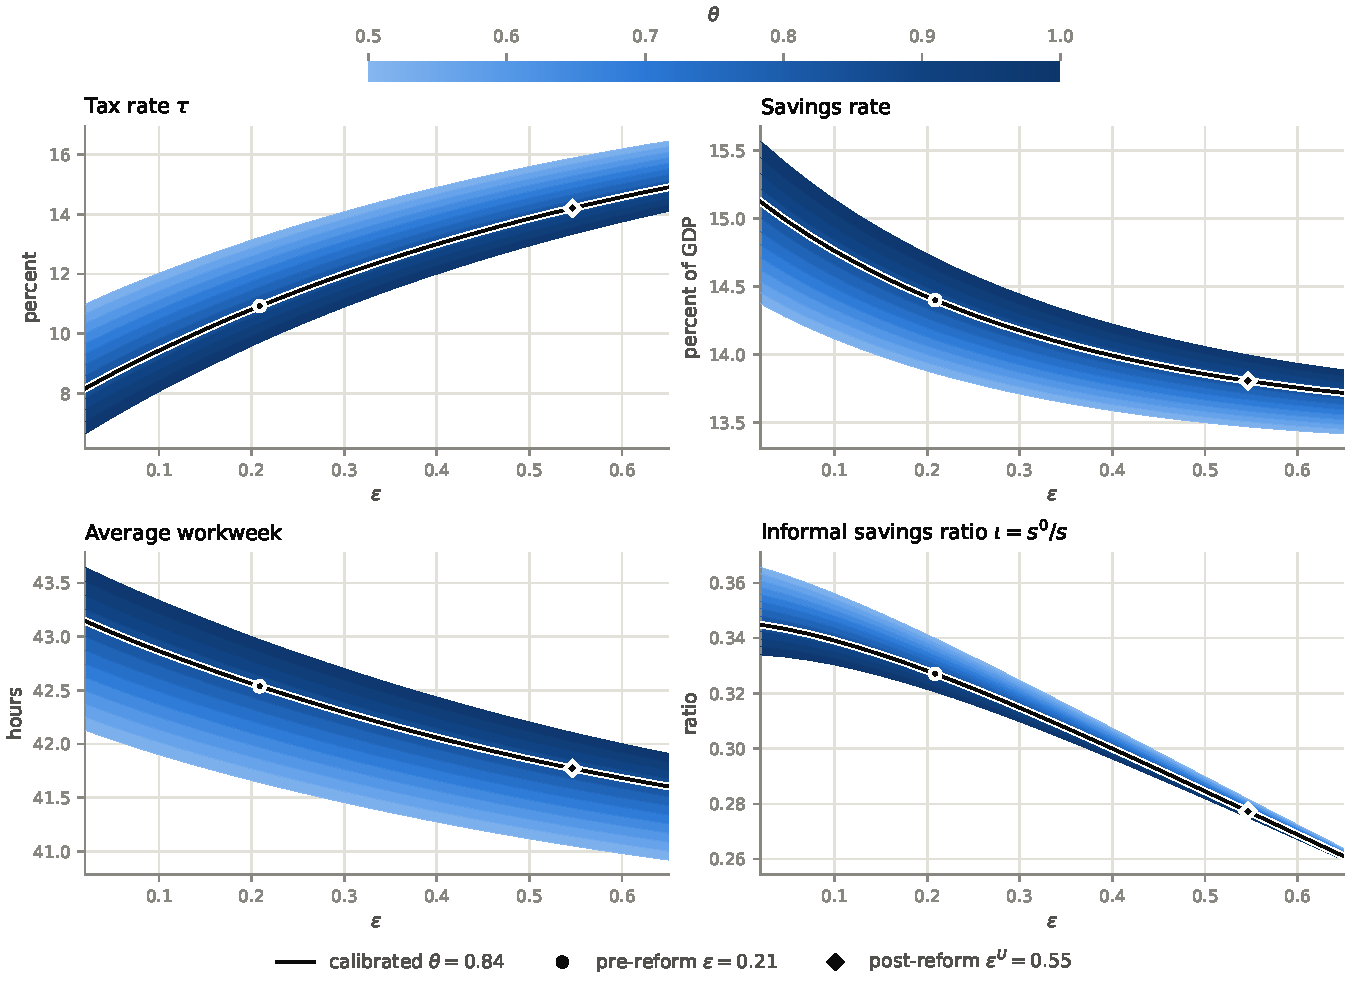
\includegraphics[width=\linewidth]{Figs/ARG_LOG_FourInOne.pdf}
\begin{tablenotes}[flushleft]\footnotesize
    \item[] \textit{Note:} The savings rate is savings relative to GDP.
\end{tablenotes}
\end{threeparttable}
\end{figure}

\smalltitle{The effect of the intertemporal elasticity of substitution.}
Since the environment has no uncertainty, we read the parameter $\rho$ of CRRA preferences as the intertemporal elasticity of substitution (IES). The evidence on its size is inconclusive,\footnote{Estimates from aggregate consumption data are low, which \textcite{Guvenena1} reconciles with higher values from output and wealth data through limited asset market participation, and asset-pricing models with Epstein--Zin preferences and long-run or disaster risk require an IES above one \parencite{BansalYa1,Barroa1}.} and we keep logarithmic utility as the benchmark. Table \ref{table:Argentina:funcOfRho} repeats the reform with the pre-reform economy recalibrated at each $\rho$, and figure \ref{fig:ARG:EffectOfCRRA} in appendix \ref{app:EPH} traces the effects in 2010 and 2040 across $\rho$. Below an IES of one the effects are dampened: at $\rho = 0.5$ the tax rate rises by only 0.2 p.p.\ in 2010, a small fraction of the observed rise in spending, and the savings rate barely moves. The reason for this is that with a low IES the young resist taxation more strongly, so the recalibrated economy needs a larger political weight of the old and responds less to a change in benefits. For $\rho$ between 1 and 2 the results stay close to the log benchmark: the tax rate rises by 1.2 to 1.3 p.p.\ in 2010 and by 2.0 to 2.1 p.p.\ by 2040, the workweek shortens by about 0.15 hours, and the fall in the savings rate shrinks from 0.3 to 0.2 p.p.\ of GDP between $\rho = 1$ and $\rho = 2$. Since \textcite{Ruffo} find that the amnesty reduced savings, we regard $\rho \in [1,2]$ as the more plausible range.

%% GENERATED by python/paper/build.py from results/ -- do not edit by hand.
%% Rebuild:  .venv\Scripts\python.exe python\paper\build.py --only Argentina_funcOfRho
%% Source:   results/shocks/universal_match_rho*_commonX.csv
\begin{table}[!htb]
\centering
\begin{threeparttable}
\caption{Pension system reform, year 2010, function of $\rho$}
\label{table:Argentina:funcOfRho}
\begin{tabular}{lccc}
\toprule
\textbf{Scenario} & \textbf{Tax rate} & \textbf{Change in savings rate} & \textbf{Avg. workweek (hours)} \\
\midrule 
Pre-reform & 10.92\% & -- & 42.54 \\[1ex]
Post-reform, $\rho$ = 0.5 & 11.11\% & $-0.04$ p.p. & 42.52 \\[1ex]
% Post-reform, $\rho$ = 0.6 & 11.51\% & $-0.16$ p.p. & 42.47 \\[1ex]
% Post-reform, $\rho$ = 0.7 & 11.79\% & $-0.23$ p.p. & 42.44 \\[1ex]
% Post-reform, $\rho$ = 0.8 & 11.97\% & $-0.26$ p.p. & 42.42 \\[1ex]
% Post-reform, $\rho$ = 0.9 & 12.10\% & $-0.28$ p.p. & 42.40 \\[1ex]
Post-reform, $\rho$ = 1.0 & 12.17\% & $-0.28$ p.p. & 42.39 \\[1ex]
% Post-reform, $\rho$ = 1.1 & 12.22\% & $-0.28$ p.p. & 42.39 \\[1ex]
% Post-reform, $\rho$ = 1.2 & 12.24\% & $-0.28$ p.p. & 42.39 \\[1ex]
% Post-reform, $\rho$ = 1.3 & 12.25\% & $-0.27$ p.p. & 42.38 \\[1ex]
% Post-reform, $\rho$ = 1.4 & 12.25\% & $-0.26$ p.p. & 42.38 \\[1ex]
% Post-reform, $\rho$ = 1.5 & 12.24\% & $-0.25$ p.p. & 42.38 \\[1ex]
% Post-reform, $\rho$ = 1.6 & 12.23\% & $-0.24$ p.p. & 42.39 \\[1ex]
% Post-reform, $\rho$ = 1.7 & 12.21\% & $-0.23$ p.p. & 42.39 \\[1ex]
% Post-reform, $\rho$ = 1.8 & 12.20\% & $-0.22$ p.p. & 42.39 \\[1ex]
% Post-reform, $\rho$ = 1.9 & 12.17\% & $-0.21$ p.p. & 42.39 \\[1ex]
Post-reform, $\rho$ = 2.0 & 12.14\% & $-0.20$ p.p. & 42.39 \\[1ex]
\bottomrule
\end{tabular}
\begin{tablenotes}[flushleft]
\footnotesize
\item[] \textit{Note:} The reform permanently shifts $\epsilon = 1-\theta + \theta \eta_1 h_1/h$. Each $\rho$ is separately recalibrated to the same pre-reform targets, so the pre-reform tax rate and workweek are common to every $\rho$. The savings rate is savings relative to GDP; its pre-reform level is not targeted (the capital--output ratio is) and varies with $\rho$, so each post-reform row reports the change against its own $\rho$'s pre-reform level in percentage points.
\end{tablenotes}
\end{threeparttable}
\end{table}


Section \ref{sec:oecd} turns to three rich economies whose coverage is nearly universal, so that their pension designs differ only in the Bismarckian index $\theta$.
